\chapter{Технологический раздел}

\section{Средства реализации}

% В настоящее время существует множество систем управления базами данных, работающих на основе реляционной модели. Среди самых распространенных \cite{most_popular} выделяют MySQL \cite{mysql}, PostgreSQL \cite{postgresql} и замыкает тройку лидеров SQLite \cite{sqlite}. Их особенности:
% \begin{enumerate}
% 	\item MySQL. Среди достоинств данной СУБД можно выделить простой синтаксис, высокую безопасность и масштабируемость, поддержку большей части функционала SQL.
% 	\item PostgreSQL. В рамках использования этой СУБД имеется возможность помимо встроенного SQL использовать различные дополнения, отличается поддержкой форматов csv и json, но оперирует большим объемом ресурсов.
% 	\item SQLite. Очевидными достоинствами является компактность базы данных, которая состоит из одного файла, и легкая переносимость. Но данная СУБД совершенно не подходит для больших БД, а также не поддерживает управление пользователями.
% \end{enumerate}

При реализации проекта будет использована PostgreSQL\cite{postgresql}, поскольку эта 
СУБД является реляционной и обладает достаточным набором инструментов для решения поставленной задачи.

В качестве используемого языка программирования выбран Python\cite{python}, по причине его тесной интеграции с PostgreSQL, простоте синтаксиса и высокой скорости развёртывания REST-приложений на нём. 

Для реализации REST API был выбран фреймворк Flask\cite{flask}, так как он достаточно прост в освоении и позволяет быстро создать полноценное REST-приложение.

Для реализации ORM\cite{orm} использовался инструментарий 
SQLAlchemy~\cite{sqlalchemy} по причине его тесной интеграции с Flask. Для тестирования приложения была выбрана утилита Postman\cite{postman}, потому что она обладает графическим интерфейсом и в то же время предоставляет широкий набор возможностей для тестирования API приложения.


\section{Создание базы данных}

В соответствии с выбранной СУБД и спроектированной базой данных было осуществлено создание БД и ее сущностей. Реализация представлена в приложении А, листинг \ref{create}.

В предыдущем разделе был спроектирован триггер AFTER на создание новой заявки в системе. Код его создания представлен в листинге \ref{trigger_code}

\captionsetup{singlelinecheck = false, justification=raggedright}
\begin{lstlisting}[language=sql, caption=Реализация триггера AFTER, label=trigger_code]
create trigger updateRatingTrigger
    after update of id_first, id_second, id_third
    on hackathons
    for each row
execute function updateRating();

\end{lstlisting}
\captionsetup{singlelinecheck = false, justification=centering}

Для этого триггера была написана соответствующая функция с помощью
PL/pgSQL \cite{plpgsql} -- процедурного расширения языка SQL, 
используемого в \newline СУБД PostgreSQL. Код функции представлен в листинге \ref{trigger_func}.

\captionsetup{singlelinecheck = false, justification=raggedright}
\begin{lstlisting}[language=sql, caption=Реализация функции updateRating(), label=trigger_func]

create or replace function updateRating()
    returns trigger as
$$
begin
    call updateTeamParticipantsRating(new.id_first, 3);
    call updateTeamParticipantsRating(new.id_second, 2);
    call updateTeamParticipantsRating(new.id_third, 1);

    call updateTeamRating(new.id_first);
    call updateTeamRating(new.id_second);
    call updateTeamRating(new.id_third);

end
$$
    language plpgsql;
    
create function updateTeamParticipantsRating(arg_team_id integer, 
rating_change integer) returns void
    language plpgsql
as
$$
begin
    update ratings
    set rating = rating + rating_change
    where id = (select id from t_p_list where team_id = arg_team_id);
end
$$;

create function updateteamrating(arg_team_id integer) returns void
    language plpgsql
as
$$
begin
    update teams
    set rating = (select sum(rating)
                  from ratings
                       join t_p_list on ratings.part_id = t_p_list.part_id
                  where t_p_list.team_id = arg_team_id)
    where id = arg_team_id;
end;
$$;

\end{lstlisting}
\captionsetup{singlelinecheck = false, justification=centering}

\section{Создание ролей и выделение им прав}

В конструкторском разделе была разработана ролевая модель, в которой выделены следующие роли:
\begin{itemize}
	\item Participant -- участник;
	\item Captain -- капитан;
	\item Organizer -- организатор;
    \item Administrator -- администратор.
\end{itemize}

Соответствующий этой ролевой модели сценарий создания ролей и выделения им прав представлен на листинге \ref{roles}.

\captionsetup{singlelinecheck = false, justification=raggedright}
\begin{lstlisting}[language=sql, caption=Создание ролей и выделение им прав, label=roles]
create user "admin" password 'admin';
create user "organizer" password 'organizer';
create user "captain" password 'captain';
create user "participant" password 'participant';

grant select on teams, hackathons, ratings, 
h_t_list, t_p_list to "participant";
grant insert on requests to "participant";

grant select on teams, hackathons, ratings, 
h_t_list, t_p_list to "captain";
grant insert on requests to "captain";
grant update on Teams to "captain";

grant select on teams, hackathons, ratings, 
h_t_list, t_p_list to "organizer";
grant insert on requests to "organizer";
grant update, delete on Hackathons to "organizer";

alter role "admin" superuser;
\end{lstlisting}
\captionsetup{singlelinecheck = false, justification=centering}

\section{Наполнение базы данных}

В ходе генерации данных было создано 5 пользователей типа "Администратор", 100 типа "Организатор" и 1000 типа "Участник". Было создано 200 команд, по которым случайным образом были распределены участники и назначен капитан. Кроме того, было создано 100 хакатонов, команды-участники были назначены случайно. Значения полей таблиц были получены случайным образом в соответствии с описанными типами данных. 

Выгрузка значений из электронных таблиц в базу данных представлен в приложении А, листинг \ref{fill}.


\section{Описание интерфейса приложения}
Приложение разрабатывалось как микросервис, доступ к которому происходит при помощи RestAPI \cite{restapi}. Схема приложения представлена на рисунке \ref{app_architecture}.

\begin{figure}[H]
	\begin{center}
		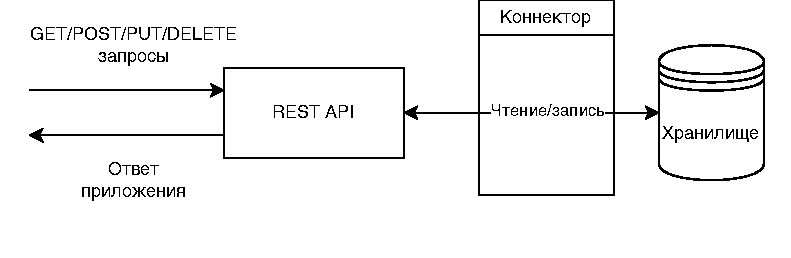
\includegraphics[page=1,scale=1]{assets/app_architecture.drawio.pdf}
	\end{center}
	\caption{Схема приложения}
	\label{app_architecture}
\end{figure}

Для доступа к приложению был создан ряд HTTP-запросы, полный список которых содержится в приложении Б. В данном разделе приведены некоторые из них:

\begin{itemize}
    \item POST (<</login>>) -- авторизация в приложении. При этом логин и пароль передаются в заголовке к запросу согласно методу BasicAuth\cite{basicauth};
    \item GET (<</hackathons>>) -- получить данные о всех хакатонах;
    \item GET (<</hackathon/<id> >>) -- получить данные о хакатоне с идентификатором id;
    \item GET (<</hackathons/<id>/teams>>) -- получить данные о командах, 
    участвующих в хакатоне;
    \item DELETE (<</hackathons/<id> >>) -- удалить хакатон. Доступно только администратору и создателю хакатона;
    \item GET (<</teams/places\_available>>) -- получить список команд со свободными местами;
    \item GET (<</teams/<id>/participants>>) -- получить список участников команды;
    \item POST (<</teams>>) -- создать команду. Доступно только администратору;
    \item POST (<</requests>>) -- подать заявку.
\end{itemize}

POST запросы требуют наличия у них тела в формате JSON\cite{json}. Ответ возвращается также в данном формате.


\section{Примеры работы}
В качестве демонстрации примеров работы были выбраны следующие пользовательские сценарии:

\begin{itemize}
    \item регистрация пользователя;
    \item авторизация пользователя;
    \item создание заявки на создание команды;
    \item одобрение заявки администратором;
    \item получение данных о будущих хакатонах.
\end{itemize}

Примеры запросов по данным сценариям и результаты их обработки представлены на рисунках \ref{ex-signup} - \ref{ex-future}

\begin{figure}[H]
	\begin{center}
		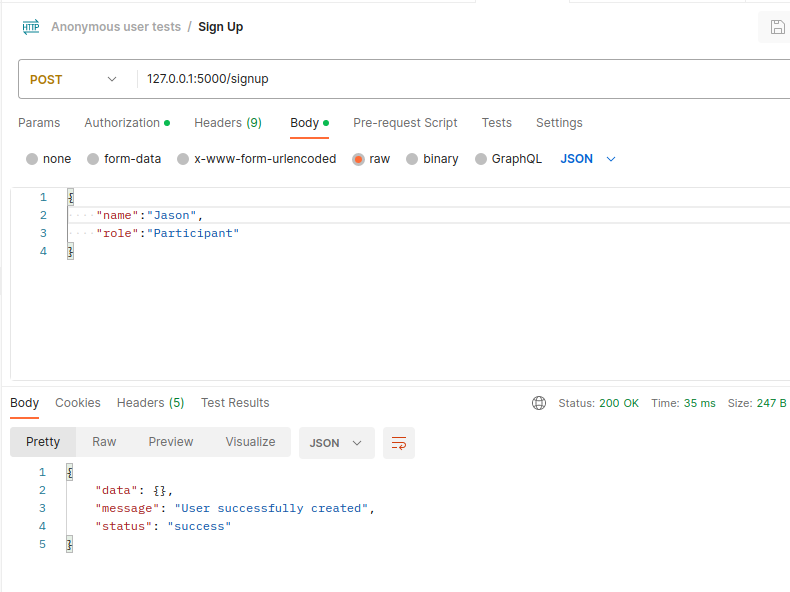
\includegraphics[page=1,scale=0.5]{assets/ex-signup.png}
	\end{center}
	\caption{Регистрация пользователя}
	\label{ex-signup}
\end{figure}

\begin{figure}[H]
	\begin{center}
		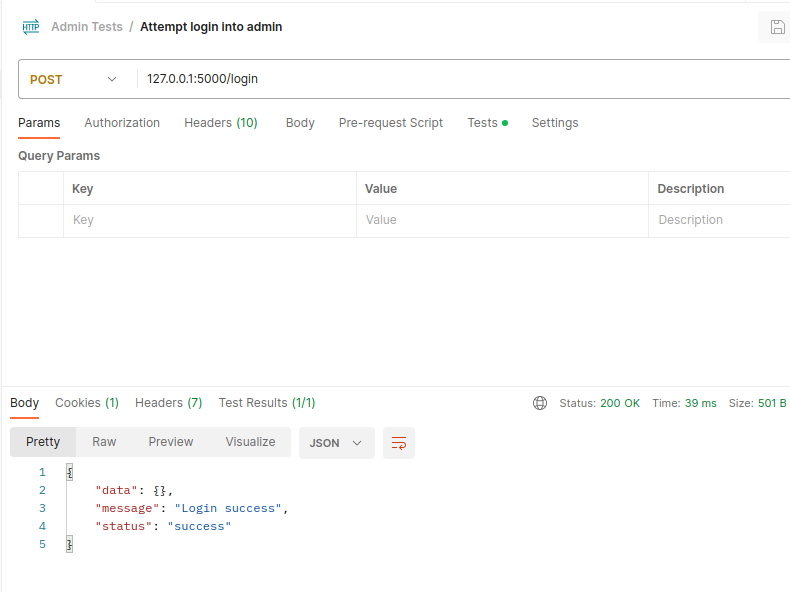
\includegraphics[page=1,scale=0.5]{assets/ex-signin.png}
	\end{center}
	\caption{Авторизация пользователя}
	\label{ex-signin}
\end{figure}

\begin{figure}[H]
	\begin{center}
		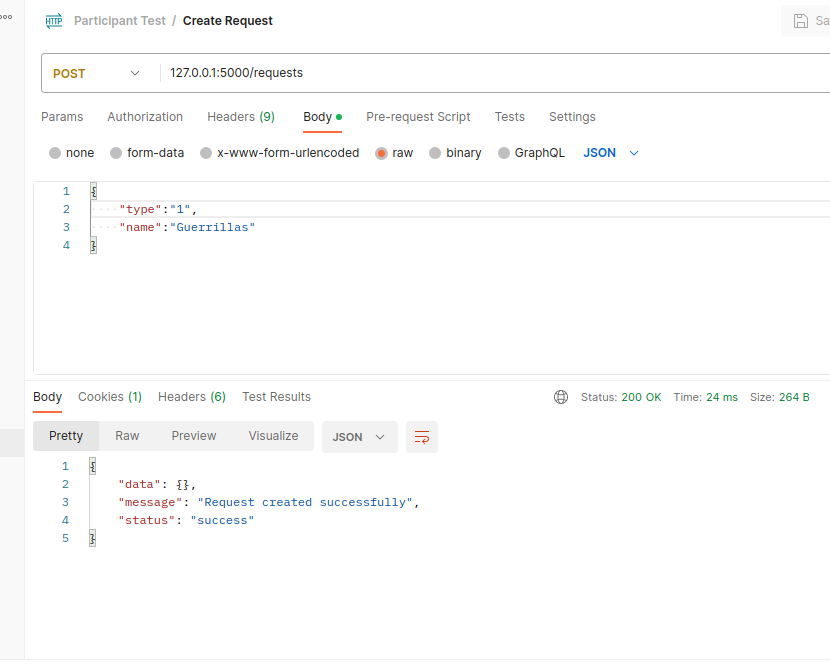
\includegraphics[page=1,scale=0.5]{assets/ex-create.png}
	\end{center}
	\caption{Создание заявки на создание команды}
	\label{ex-create}
\end{figure}

\begin{figure}[H]
	\begin{center}
		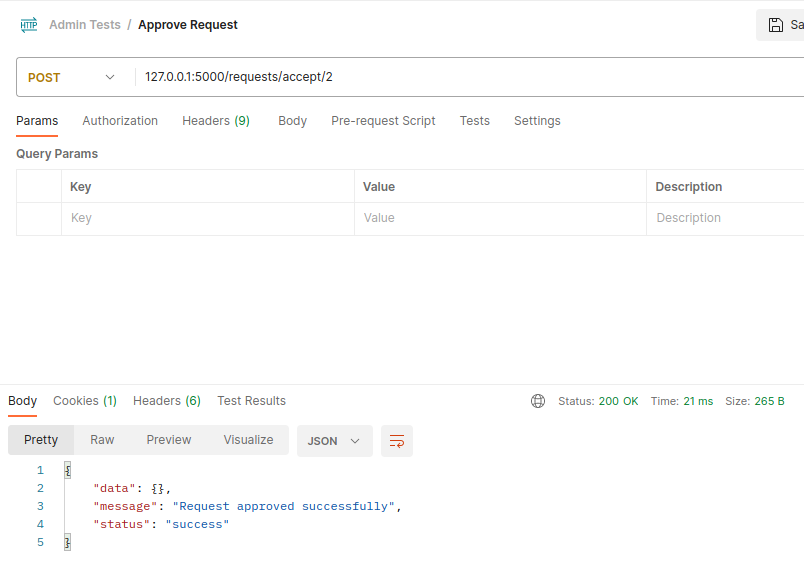
\includegraphics[page=1,scale=0.5]{assets/ex-approve.png}
	\end{center}
	\caption{Одобрение заявки администратором}
	\label{ex-approve}
\end{figure}

\begin{figure}[H]
	\begin{center}
		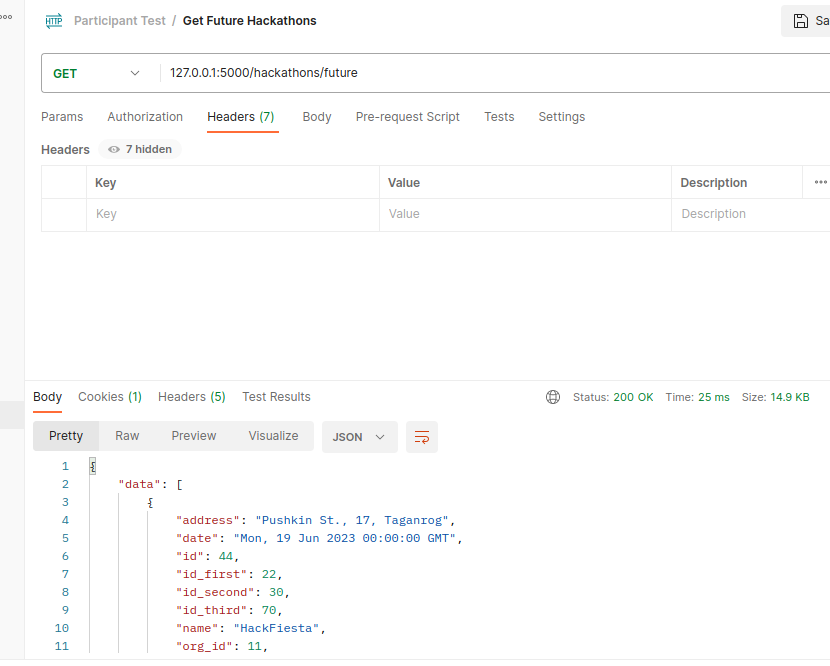
\includegraphics[page=1,scale=0.5]{assets/ex-future.png}
	\end{center}
	\caption{Получение данных о будущих хакатонах}
	\label{ex-future}
\end{figure}

\section{Нагрузочное тестирование}
В данном подразделе было выполнено нагрузочное тестирование для оценки быстродействия разработанного приложения при различном числе одновременно посылающих запросы пользователей.


Были исследованы следующие пользовательские сценарии:
\begin{enumerate}[label={\arabic*)}]
    \item получение данных о будущих хакатонах;
    \item получение данных о всех хакатонах;
    \item получение списка команд со свободными местами, данных о будущих хакатонах и отправка заявки на вступление в команду.
\end{enumerate}

Нагрузочное тестирование проводилось следующим образом: на протяжении 400 секунд число пользователей равномерно увеличивалось от 1 до 400 (то есть, каждую секунду подключался один дополнительный пользователь). Пользователи отправляли сервер

Сервер во время обработки запросов был запущен на ПК со следующими характеристиками:
\begin{itemize}
    \item RAM: 8 Гбайт DDR4;
    \item ЦПУ: AMD Ryzen 5 3500U \cite{amd};
    \item ОС: Ubuntu 20.04 \cite{ubuntu}.
    \end{itemize}

При проведении тестирования на ПК были запущены только сервисы ОС, сервер приложения и ПО для проведения тестирования -- Apache JMeter 5.5 \cite{jmeter}. Во время тестирования ПК был подключен к сети электропитания.


\subsection{Сценарий №1}

Данный сценарий состоит из следующих запросов:

\begin{enumerate}[label={\arabic*)}]
    \item POST (<</login>>);
    \item GET (<</hackathons/future>>);
    \item POST (<</logout>>).
\end{enumerate}

На графике \ref{test1_1} показаны результаты тестирования по сценарию №1 на количестве пользователей от 1 до 100, а на \ref{test1_2} -- от 1 до 400.

\begin{figure}[H]
	\begin{center}
		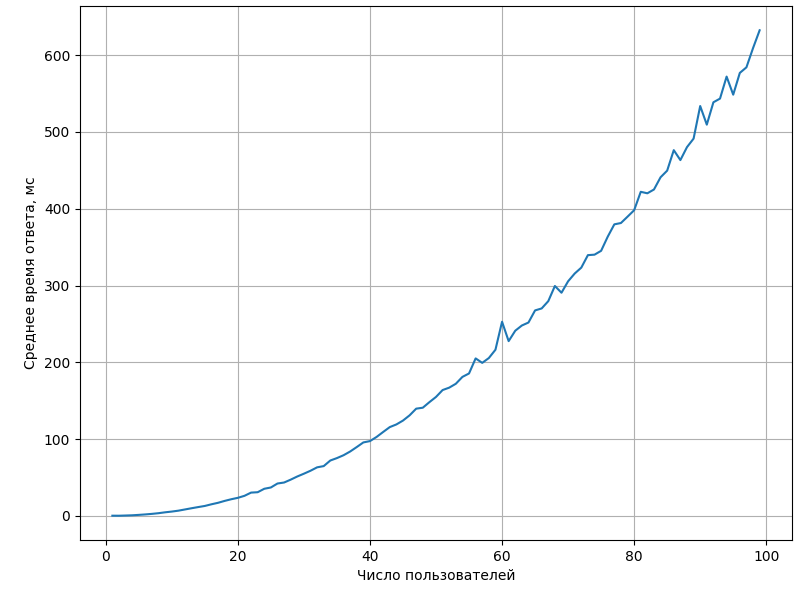
\includegraphics[page=1,scale=0.8]{assets/exp1_100.png}
	\end{center}
	\caption{Тестирование по сценарию №1, 100 пользователей}
	\label{test1_1}
\end{figure}

\begin{figure}[H]
	\begin{center}
		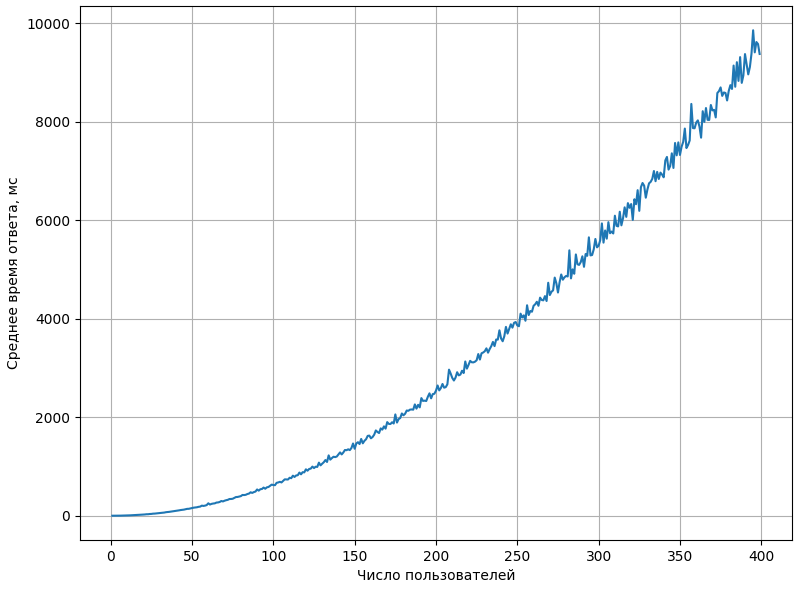
\includegraphics[page=1,scale=0.8]{assets/exp1_400.png}
	\end{center}
	\caption{Тестирование по сценарию №1, 400 пользователей}
	\label{test1_2}
\end{figure}

Из графиков видно, что при числе пользователей до 100 среднее время выполнения сценария не превышает 700 мс, однако уже при 170 пользователях время ожидания ответа приближается к 2 секундам и увеличивается вплоть до 10 секунд при 400 пользователях.

\subsection{Сценарий №2}

В ходе пользовательского сценария №2 выполняются следующие запросы:

\begin{enumerate}[label={\arabic*)}]
    \item POST (<</login>>);
    \item GET (<</hackathons>);
    \item GET (<</hackathons/future>);
    \item GET (<</teams>>);
    \item POST (<</logout>>).
\end{enumerate}

Результаты тестирования представлены на рисунках \ref{test2_1} и \ref{test2_2}.


\begin{figure}[H]
	\begin{center}
		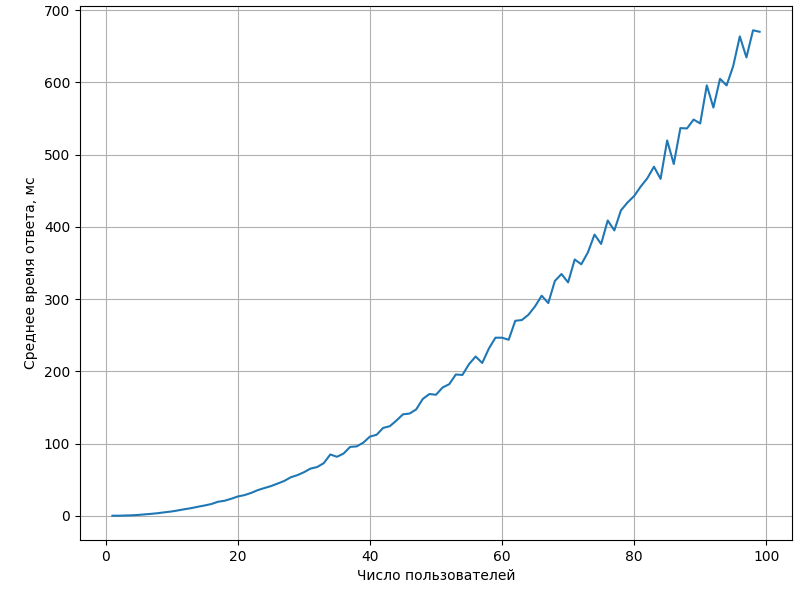
\includegraphics[page=1,scale=0.8]{assets/exp2_100.png}
	\end{center}
	\caption{Тестирование по сценарию №2, 100 пользователей}
	\label{test2_1}
\end{figure}

\begin{figure}[H]
	\begin{center}
		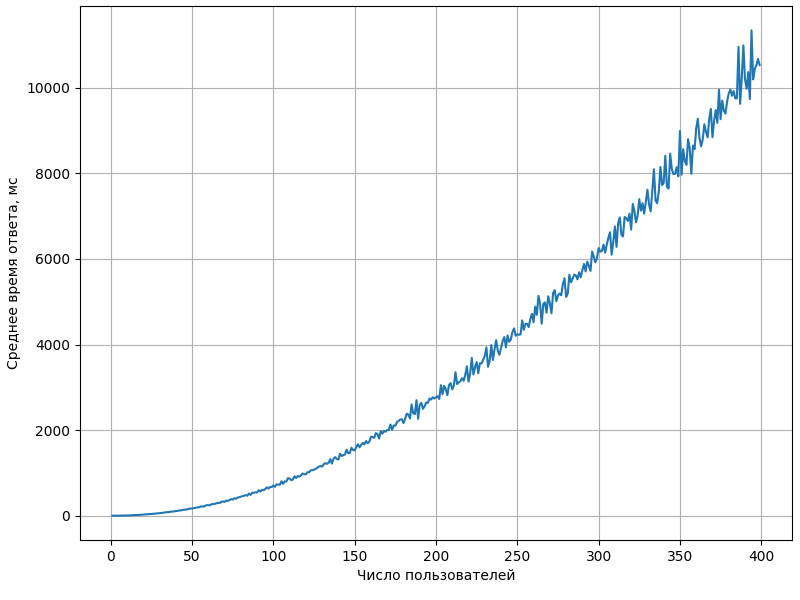
\includegraphics[page=1,scale=0.8]{assets/exp2_400.png}
	\end{center}
	\caption{Тестирование по сценарию №2, 400 пользователей}
	\label{test2_2}
\end{figure}

Из графиков видно, что добавление двух дополнительных GET запросов привело к увеличению времени ожидания ответа от сервера на 5-10\% в зависимости от числа пользователей. 


\subsection{Сценарий №3}

Данный сценарий состоит из следующих запросов:

\begin{enumerate}[label={\arabic*)}]
    \item POST (<</login>>);
    \item GET (<</hackathons>);
    \item GET (<</hackathons/future>>);
    \item GET (<</teams>>);
    \item POST (<</requests>>);
    \item POST (<</logout>>).
\end{enumerate}

Сценарий №3 содержит запросы из Сценария №2, к которым был добавлен POST запрос. В ходе его выполнения каждый пользователь создаёт заявку, данные о которой сохраняются на сервере. 

\begin{figure}[H]
	\begin{center}
		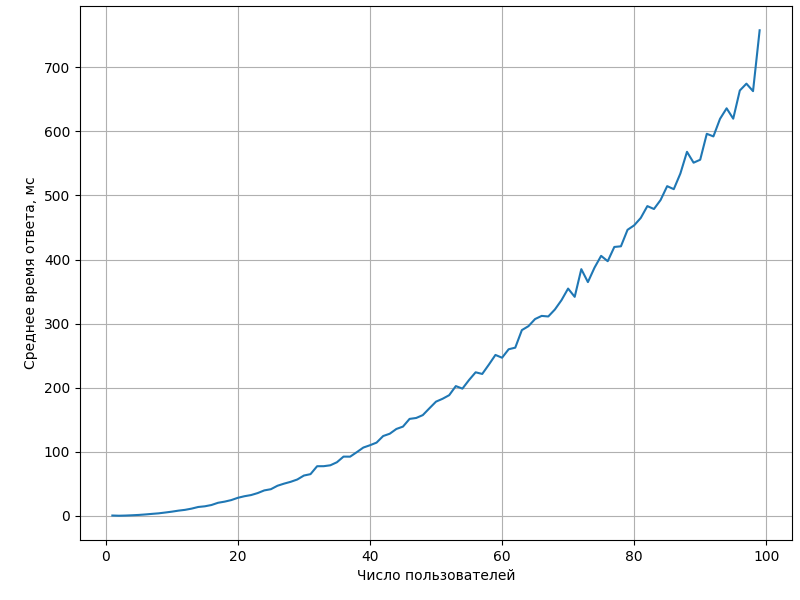
\includegraphics[page=1,scale=0.8]{assets/exp3_100.png}
	\end{center}
	\caption{Тестирование по сценарию №3, 100 пользователей}
	\label{test1_1}
\end{figure}

\begin{figure}[H]
	\begin{center}
		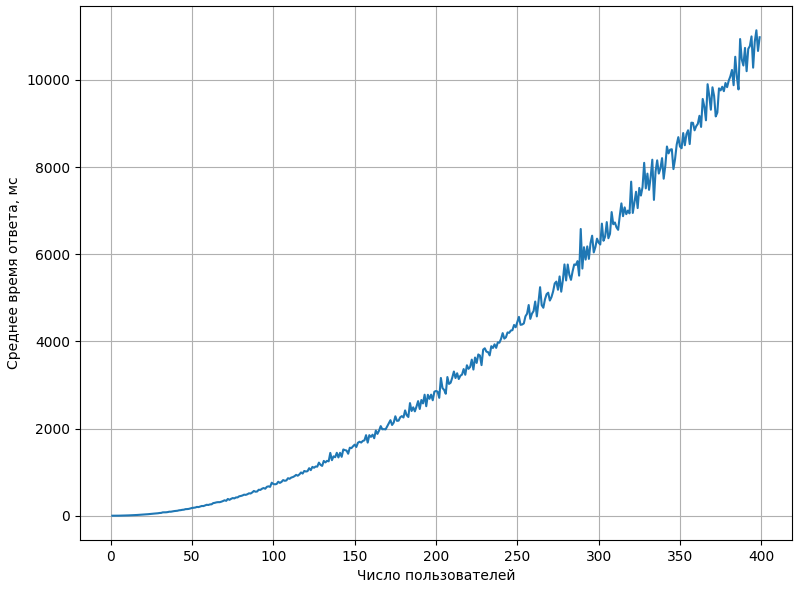
\includegraphics[page=1,scale=0.8]{assets/exp3_400.png}
	\end{center}
	\caption{Тестирование по сценарию №3, 400 пользователей}
	\label{test1_2}
\end{figure}

В ходе тестирования по данному сценарию было выявлено дальнейшее увеличение
времени ответа на 5-10\%.

\newpage
\section{Вывод из раздела}
В данном разделе был сделан выбор СУБД и средств реализации, описано создание БД, триггера, ролей с выделением прав. Также были представлены описание генерации данных для наполнения базы и примеры работы ПО и проведено нагрузочное тестирование, в ходе которого было выяснено,что созданное приложение на вышеуказанном оборудовании достаточно плохо справляется с ситуацией, в которой достаточно большое ($\geq 150$) число пользователей одновременно посылает запросы. При этом уже начиная с 400 пользователей время ожидания ответа от приложения составляет порядка десяти секунд, что достаточно сильно усложняет работу пользователя \cite{attention}.